\documentclass[conference]{IEEEtran}
\IEEEoverridecommandlockouts

\usepackage{amssymb}
\usepackage[tight,footnotesize]{subfigure}
\usepackage[dvips]{graphicx}
\DeclareGraphicsExtensions{.eps}

\begin{document}

\title{Efficient Access Protocols for High Storage RFID}

\author{
\IEEEauthorblockN{Victor K.Y. Wu$^*$ and Nitin H. Vaidya}
\IEEEauthorblockA{Department of Electrical and Computer Engineering\\
University of Illinois at Urbana-Champaign\\
Email: \{vwu3, nhv\}@illinois.edu}
\thanks{$^*$This work is supported by NSF grant  CNS-0519817.}
}

\maketitle

\section{Introduction}
Passive UHF RFID tags are increasing in storage sizes (up to 32 kilobytes \cite{web:tego}), allowing them to form distributed storage mechanisms with very little maintenance cost (they are passive, and easily replaceable, cost-wise).  This type of distributed storage is characterized by it's inherent randomness (tags may come and go, not be scanned, or just fail).  In this work, we provide motivating applications and design goals for high storage passive RFID.  We consider several protocols to read from and write to such a distributed storage mechanism, and investigate preliminary performance results.  Finally, we conclude and explain our future research directions.

\section{Motivations and design goals}
\subsection{Applications}
One application is enhancing the already existing use of passive RFID in warehousing and supply chain management.  Tags are attached to pallets (and sometimes even individual items) of goods.  With large tag storage sizes, we can record extensive information, such as histories of pallet locations in the supply chain, to be read later.  Since information is stored \emph{inline}, within the tags themselves, interrogators do not have to look up databases to learn information about tagged items when scanning tags.  This is especially advantageous when different interrogators (at possibly different physical sites, belonging to different entities in the supply chain) do not have access to the same database.

High storage passive RFID can also be used in consumer applications.  For example, consider a digital whiteboard composed of many passive tags.  Users can read and write messages.  Tags can be added, removed, or even shuffled between different whiteboards, depending on the scenario.  Similarly, these tags can be used as personal digital notebooks.  Users can have a number of tags at home or in the office, which they read from and write to.  They can be traded between friends and coworkers as a way to communicate.  Furthermore, the tags can be combined in a variety of ways for different types of interactions, leading to aggregate-level (multi-tag) read and writing.

\subsection{Design goals}
These motivating applications point toward certain design goals.  In particular, since we know that tags may randomly move in and out of a system (e.g. a pallet, a digital whiteboard, or an office desk) or just fail, we do not want to keep track of each individual tag.  Furthermore, since different and non-communicating interrogators may access the same tags, we do not want interrogators to save any state information (such as number of tags or access times).  Any state information should be stored in the tags themselves (if at all).

We want an interrogator to read the newest information written to a system of tags from a previous interrogator, because the freshest data is often the most relevant.  In many applications, this may be a ``best effort" design.  For example, if the tags carrying the newest information leave, the interrogator may be only able to read the second newest information.  A secondary goal is reading the rest of the history of previous interrogator writes.  In particular, we place less weight on recovering information further in the past.  This points to the design goals in writing to a system of tags.  

We want to write to empty tags if they exist.  Otherwise, if we are forced to overwrite previous information, we want to replace the oldest data in the system.  For the same reasons above, writing may also be a best effort design.  Another goal related to writing is redundancy.  We may want to encode and store information in multiple tags, to combat tag failures and tag movement.  Finally, reading and writing should be as fast as possible.  

One further design goal that is not directly addressed in this work (but is the subject of future work) is offering user-defined priorities to data.  (Right now, newer information is assumed to have higher priority.)

\section{Protocols}
In our proposed protocols, we consider only a single interrogator accessing a system of tags.  In future work, we consider extending our ideas to allow multiple interrogators to interact with a tag system simultaneously.   

\subsection{Timestamps Protocol (TP)}
In TP, we store timestamps with messages in tags.  That is, when an interrogtor writes a message to a tag, it includes a timestamp, stored locally on the tag.  Later, when an interrogator is searching for the newest message in the system, it first singulates all the tags, reading their timestamps at the same time.  (Singulation can be done using any existing protocol, such as query tree \cite{conf:Law01} or slotted aloha \cite{conf:Vogt01} based schemes.)  Then it reads the message from the tag with the newest timestamp.  Similarly, when an interrogator wants to a write a message to the system, it first singulates all the tags, reading their timestamps.  (Empty tags have no timestamps.)  The interrogator writes the message to the first empty tag it singulates.  If all the tags in the system are full, it writes to the tag with the oldest timestamp, replacing the existing message there.

We consider an extension to this protocol.  When an interrogator wants to write, only tags which are ``old" respond.  Similarly, when reading, only tags which are ``new" respond.  Whether tags are ``old" or ``new" can be determined using a variety of ways, such as the interrogator including a search time period in it's queries to the tags.  This reduces the number of tags that need to be singulated.

Another extension is trading off accuracy for access speed.  For example, we can continually keep track of the newest and oldest tags (their IDs) during singulation.  If we are satisfied early on in the singulation process (e.g. the newest and oldest timestamps discovered so far are already very new and very old, respectively), then we can stop the singulation process, saving time.  This applies to both query tree and slotted aloha schemes.  This idea can be applied to the other protocols as well.

\subsection{Pointers Protocol (PP)}
In PP, we store pointers (IDs) to the newest and oldest tag (and possibly other ordered tags) within the tags themselves.  Therefore, reading and writing is easily achieved if an interrogator learns the pointers.  Thus, the difficulty of this protocol is reading and maintaining these pointers.  For example, we may use dedicated tags to store these pointers.  However, if interrogators do not know the dedicated tags, or even worse, if the dedicated tags fail or leave, we lose the crucial pointer information.  We envision more robust solutions randomly spread pointer information in the tags, in a redundant fashion, possibly with timestamps.  When an interrogator queries the system for pointer information, tags respond, perhaps randomly, or according to how old or new they think they are.  In this sense, PP is similar to TP.

\subsection{Dynamic IDs Protocol (DIP)}
In DIP, we modify the IDs of tags dynamically.  When an interrogator wants to write a message to the system, it first issues a broadcast command to all the tags in the system, telling them to each increase it's ID by one, modulo the number of possible IDs (wrap around if necessary).  Next, the interrogator queries for the ID zero.  If it does not exist, the interrogator searches for the tag with the largest ID (querying IDs in decreasing order starting with the largest), and changes that ID to zero.  Finally, it writes to that tag.  This guarantees that the newest message is always in the ID zero tag.  Furthermore, over time, as the system is filled with messages, the oldest information is always replaced when an interrogator writes a new message.  Therefore, when an interrogator wants to read the newest message, it simply queries the ID zero tag, reading the message stored in it.  

For example, suppose the system has $5$ tags with IDs $\{0, 5, 100, 230, 244\}$.  When writing, the plus one command results in the IDs becoming $\{1, 6, 101, 231, 245\}$.  Next, since ID $0$ does not exist (learned after a query), it searches for the largest ID by querying $255, 254, \ldots$  When it reaches ID $245$, it changes the ID in that tag to $0$, and writes the message to it.  After five writes to the system, the IDs are always $\{0, 1, 2, 3, 4\}$.  The interrogator queries the ID zero tag to read the newest message.

\subsection{Timeslots Protocol (TSP)}
\subsubsection{Timeslots Protocol-Linear (TSP-L)}
In TSP-L, we write to the ``future", and read from the ``past".  We associate each possible tag ID ($\in \{0, 1, \ldots, 2^n-1\}$ for $n$ bit IDs) with a numbered time slot of constant length in a fixed overall time period.  For example, for $n = 16$ bit IDs in a $24$ hour overall time period, each time slot is $1.318359$ seconds.  Each tag also has a dedicated bit for a wrote flag, which is off by default.  The wrote flag indicates that the tag has recently been written to, and should not be written to again.

When an interrogator wants to write, it first translates the current time $t$ to the associated ID, which we call $ID_t$.  (For instance, $ID_u = 0$, for $u \in \left[0, 1.318359\right)$ seconds in our example).  Then it broadcasts $ID_t$ to all tags in the system.  Tags with smaller IDs than $ID_t$ in a small time locality set their wrote flags off.  For example, consider the interrogator broadcasting ID $4$.  If the small time locality is equivalent to $10$ time slots, then tags within that time locality in the ``past" each set it's wrote flag off (if it is not already off).  That is, tags with IDs $\{65531, \ldots, 65535, 0, 1, \ldots, 4\}$ set it's wrote flags off.  Since we only write to the future, tags in the past have their wrote flags switched off.  $24$ hours later, those tags can be written to again, since their wrote flags are off.  This broadcast of $ID_t$ effectively updates the tags of the current time.  Next, the interrogator searches ``forward in time" to find a tag that has it's wrote flag off.  That is, it queries $ID_t + 1, ID_t + 2, \ldots (\mbox{modulo } 2^n)$ until a tag with it's wrote tag off responds.  When it finds the tag, it writes to it, and sets it's wrote flag on.

When an interrogator wants to read, it first broadcasts $ID_t$ to all tags in the system, as before.  Then it searches ``backward in time" to find the newest message.  That is, it queries $ID_t, ID_t -1, \ldots (\mbox{modulo } 2^n)$ until a tag with a message responds.

\subsubsection{Timeslots Protocol-Query Tree (TSP-QT)}
TSP-QT is the same as TSP-L, except we use a different way to search forward and backward in time for the next valid tag, when writing and reading, respectively. 

Consider all possible $2^n$ IDs in binary form, organized as the leaves of a binary tree, as shown in Fig. \ref{fig:tree} (where $n = 4$).  If a tag is in the system, it's ID (in binary form) is shown in the corresponding leaf.  If the tag is absent, the node is solid.  The wrote flag for each tag is indicated by $W$.  Common ID prefixes are shown inside non-leaf nodes.  In Fig. \ref{fig:tree}, suppose that an interrogator wants to write at time $t$, and $ID_t = 0010$ (binary form).   It first broadcasts $0010$ to the system, updating the wrote flags accordingly.  Next, it searches in the future for a tag that has it's wrote flag off.  In this case, that tag has $ID = 1000$.  Instead of searching linearly, TSP-QT looks for the root of a subtree containing the node $1000$, that is in the future.  In this case, that root is $10$ (which we explain below).  The interrogator then performs query tree singulation \cite{conf:Law01} starting at this root.  The tag we are searching for, $1000$, has the smallest ID in this subtree.

To find the subtree with root $10$, the interrogator successively queries up the tree, towards the right.  Tags with matching prefixes and wrote flag off respond, just like the query tree algorithm.  Therefore, when at least one tag responds, that prefix is the root.  In particular, these two rules guarantee that the root will be located.  (1) If the current query is a left child, the next query is just the corresponding right child.  That is, just flip the last bit from $0$ to $1$.  (2) Otherwise, move up the binary tree one level, and move laterally to the right one node.  That is, if the current query has $m$ bits, strip off the last bit, and add $1$ (modulo $2^{m-1}$) to it.  This is the next query.  In our example, the order of queries to search for the root is $\{0011, 010, 011, 10\}$.

Reading in TSP-QT is similar.  We search backward in time instead.  The two rules are reversed.  That is, if the current query is a right child, the next query is the corresponding left child.  Otherwise, move up the binary tree one level, and move laterally to the left one node.


\begin{figure}
\centering
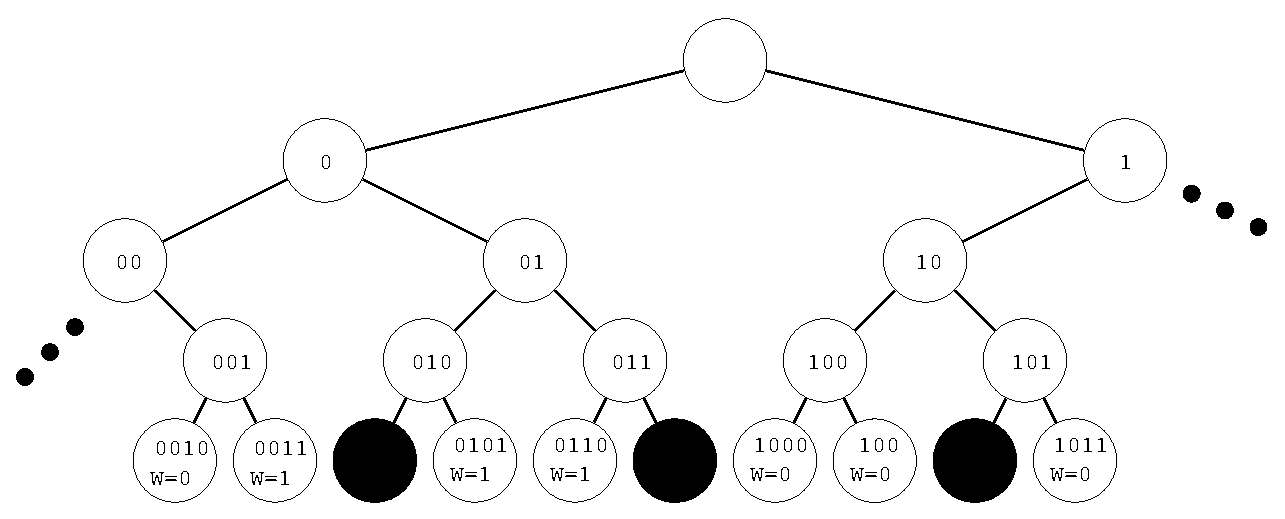
\includegraphics[width=3.5in]{query_tree.eps}
\caption{Binary tree representation of the tags in a system.  Tag IDs are the leaves.  Solid leaves indicate that the corresponding tag is not in the system.  $W$ is the wrote flag of a tag.\label{fig:tree}}
\end{figure}

\section{Preliminary performance results}

\subsection{Tags stationary}
In the first case, we consider the situation where tags remain constant in a system (such as in a warehouse pallet).  In our model, there are $N$ tags each with an ID $\in \{0, \ldots, 2^n-1\}$, where $n$ is the length of the IDs in bits.  Only one interrogator reads or writes to a system at any given time.  Once the system has reached steady state (sufficient writes to tags have occurred such that all the tags are full), we see that PP and DIP require only one query to find the newest tag to read from, and the oldest tag to write to.  In contrast, TP and TSP require multiple queries.

\subsection{Dynamic tags}
In the second case, we consider the situation where tags may arrive or leave a system.  PP and DIP are not guaranteed to work in this scenario.  (In future work, we plan to modify them for this purpose.)  Therefore, we only consider TP and TSP.  Our model is the same as before.  We seek to find the average time required to read or write to a system (in number of interrogator queries).  We see that reading and writing takes the same time.  Additionally, we assume that interrogators arrive relatively slowly, so that we can ignore the wrote flags mechanism for TSP.

We simulate TP and TSP, using $n = 16$ bits, and $N \in \{100,\ldots, 1000\}$ tags.  Results are are shown in Fig. \ref{fig:access_time}.  Note that the y-axis is in log scale.  We see TP performs poorly, since it is uses query tree to singulate all the tags.  Therefore, access time increases as the number of tags increase.  TSP-L improves as $N$ increases, since the expected difference between consecutive tag IDs of present tags in the system decreases.  Finally, TSP-QT performs the best, as this expected difference is made effectively smaller, by using the query tree algorithm on subtrees.

\begin{figure}
\centering
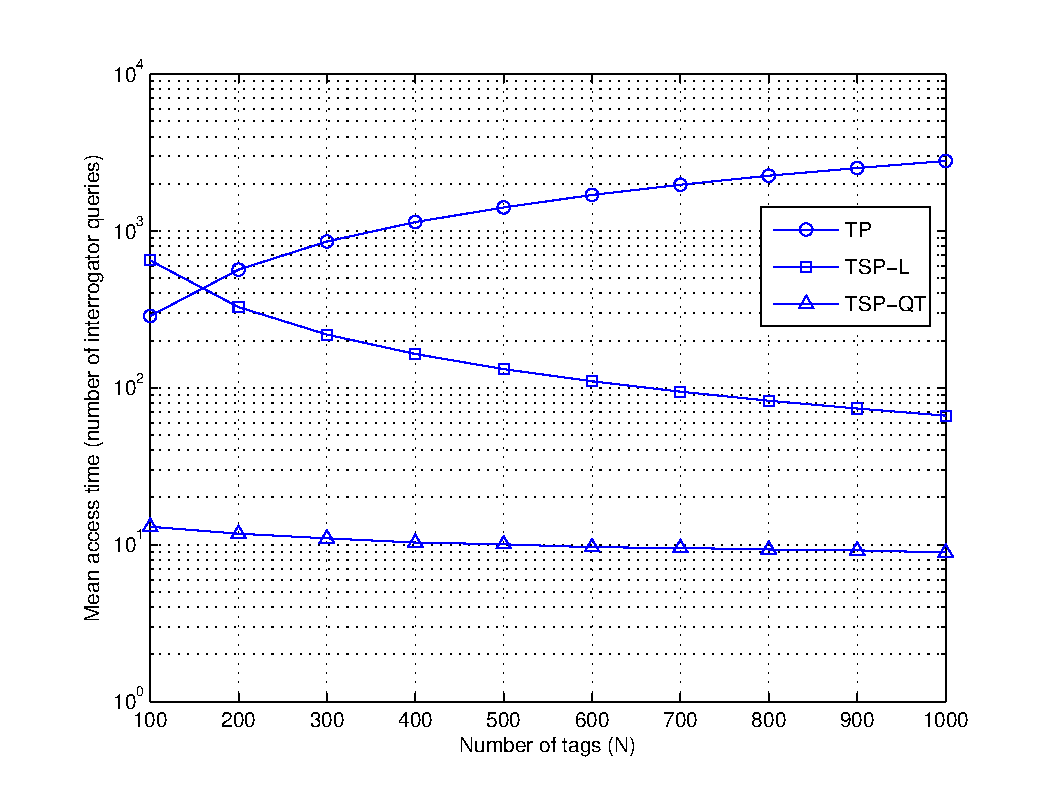
\includegraphics[width=3.5in]{access_time.eps}
\caption{Mean access times (reading or writing) for TP, TSP-L, and TSP-QT. \label{fig:access_time}}
\end{figure}

\section{Conclusion and future work}
In this work, we introduce the problem of reading and writing to a system of high storage passive RFID tags.  We consider design goals, based on motivating applications.  We consider access protocols and provide preliminary performance results.  Future work includes defining more detailed access protocols (and in which scenarios they are applicable).  We also plan to evaluate these protocols more extensively through simulations and experiments using RFID hardware.

\begin{thebibliography}{1}

\bibitem{web:tego}
``TegoChip," \emph{Tego}. [Online]. Available: http://www.tegoinc.com/products/products\_tegochip.php.

\bibitem{conf:Law01}
C. Law, K. Lee, and K.-Y. Siu, ``Efficient Memoryless Protocol for Tag Identification," in \emph{Proc. ACM International Workshop on Discrete Algorithms and Methods for Mobile Computing and Communications}, Boston, MA, Aug. 2000, pp. 75-84.

\bibitem{conf:Vogt01}
H. Vogt, ``Multiple Object Identification with Passive RFID Tags," in \emph{Proc. IEEE Conference on Systems, Man, and Cybernetics (SMC)}, Hammamet, Tunisia, Oct. 2002.


\end{thebibliography}

\end{document}


